\begin{figure}[!htb]
    \centering
    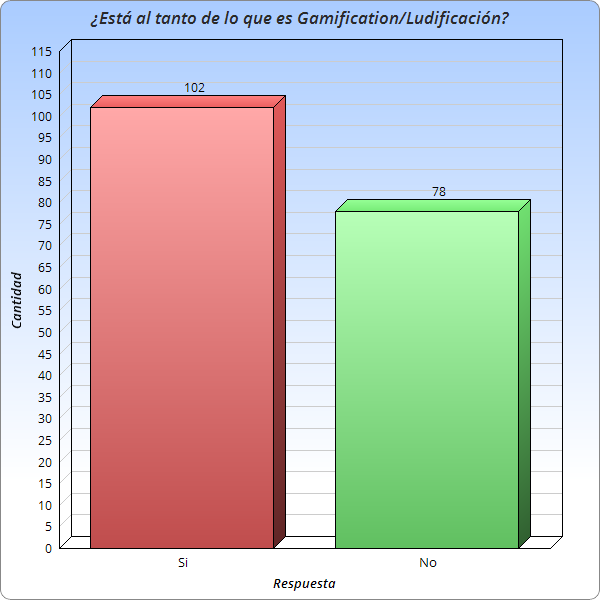
\includegraphics[width=0.6\textwidth]{images/Graficos/graf_5_1.png}
    \caption[Gráfico pregunta 3 de encuesta, conocimiento de {\gam}.]{Respuesta a pregunta $3$, conocimiento de {\gam}.}
    \label{fig:chart5.1}
    %\url{http://www.chartgo.com/get.do?id=69b1dc7d4e}
\end{figure}

\begin{figure}[!htb]
    \centering
    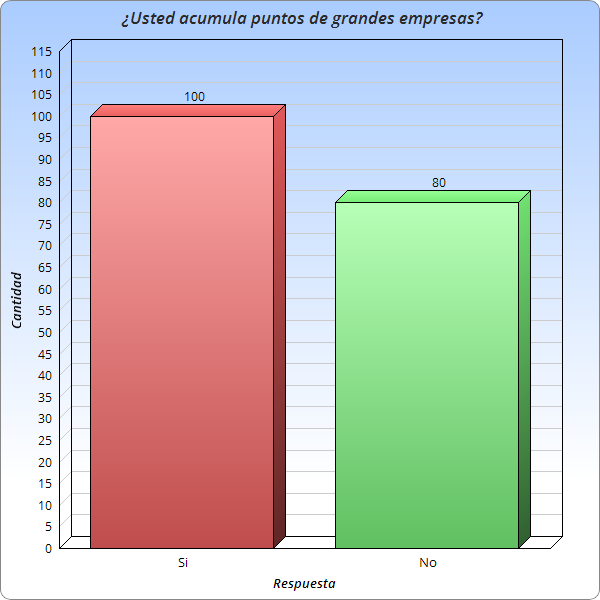
\includegraphics[width=0.6\textwidth]{images/Graficos/graf_5_2.png}
    \caption[Gráfico pregunta 4, acumulación de puntos.]{Respuesta a pregunta 4, acumulación de puntos.}
    \label{fig:chart5.2}
    %\url{http://www.chartgo.com/get.do?id=69b1dc7d4e}
\end{figure}

\begin{figure}[!htb]
    \centering
    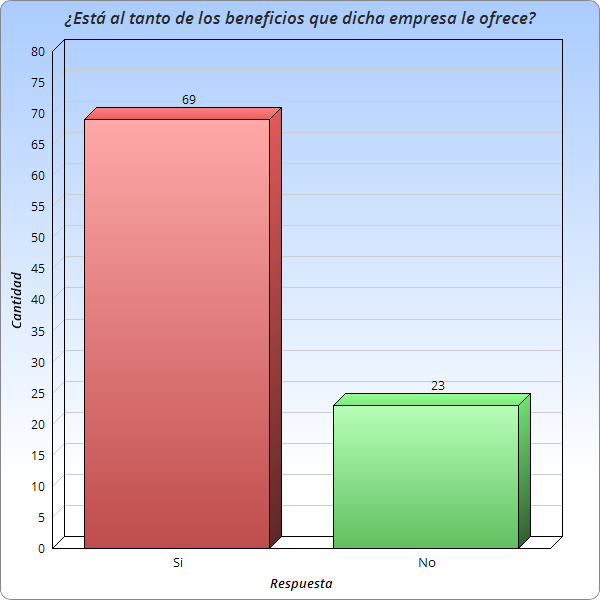
\includegraphics[width=0.6\textwidth]{images/Graficos/graf_5_3.png}
    \caption[Gráfico pregunta 5, conocimiento de beneficios.]{Respuesta a pregunta 5, conocimiento de beneficios.}
    \label{fig:chart5.3}
    %\url{http://www.chartgo.com/get.do?id=69b1dc7d4e}
\end{figure}

\begin{figure}[!htb]
    \centering
    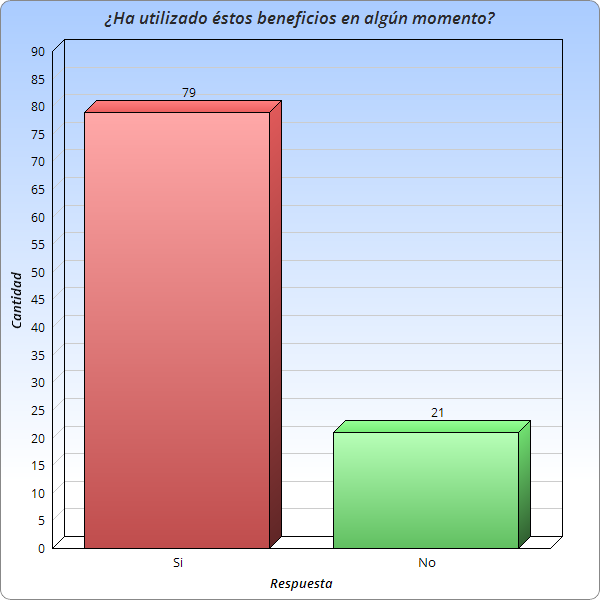
\includegraphics[width=0.6\textwidth]{images/Graficos/graf_5_4.png}
    \caption[Gráfico pregunta 6, utilización de los beneficios.]{Respuesta a pregunta 6, utilización de los beneficios.}
    \label{fig:chart5.4}
    %\url{http://www.chartgo.com/get.do?id=69b1dc7d4e}
\end{figure}

\begin{figure}[!htb]
  \centering
  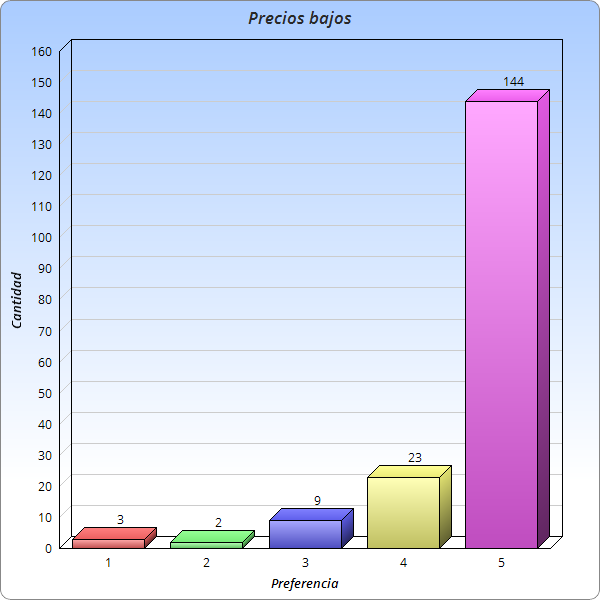
\includegraphics[width=0.6\textwidth]{images/Graficos/graf_5_5.png}
  \caption[Gráfico pregunta 7, cantidad de preferencias a beneficio de precios bajos.]{Respuesta a pregunta 7, cantidad de preferencias a beneficio de precios bajos.}
  \label{fig:chart5.5}
  %\url{http://www.chartgo.com/get.do?id=69b1dc7d4e}
\end{figure}

\begin{figure}[!htb]
  \centering
  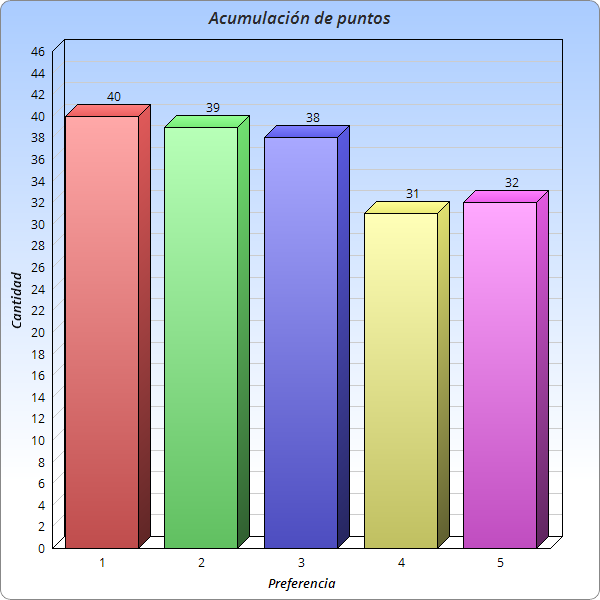
\includegraphics[width=0.6\textwidth]{images/Graficos/graf_5_6.png}
  \caption[Gráfico pregunta 7, cantidad de preferencias a beneficio de acumulación de puntos.]{Respuesta a pregunta 7, cantidad de preferencias a beneficio de acumulación de puntos.}
  \label{fig:chart5.6}
  %\url{http://www.chartgo.com/get.do?id=69b1dc7d4e}
\end{figure}

\begin{figure}[!htb]
  \centering
  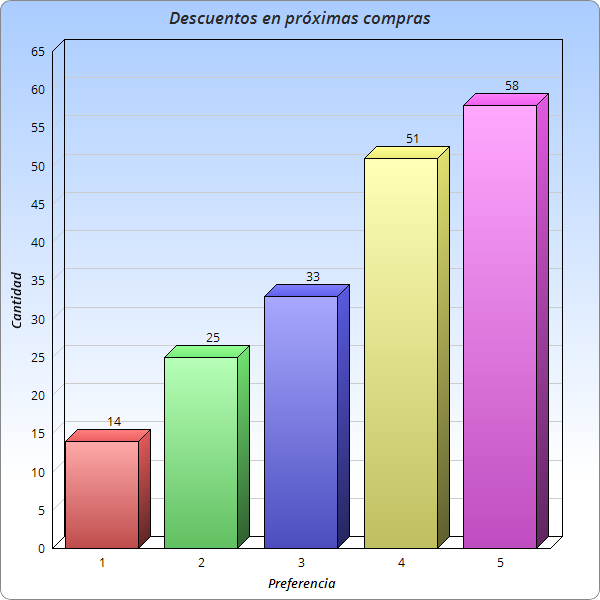
\includegraphics[width=0.6\textwidth]{images/Graficos/graf_5_7.png}
  \caption[Gráfico pregunta 7, cantidad de preferencias a beneficio de descuento en
próximas compras.]{Respuesta a pregunta 7, cantidad de preferencias a beneficio de descuento en
próximas compras.}
  \label{fig:chart5.7}
  %\url{http://www.chartgo.com/get.do?id=69b1dc7d4e}
\end{figure}

\begin{figure}[!htb]
  \centering
  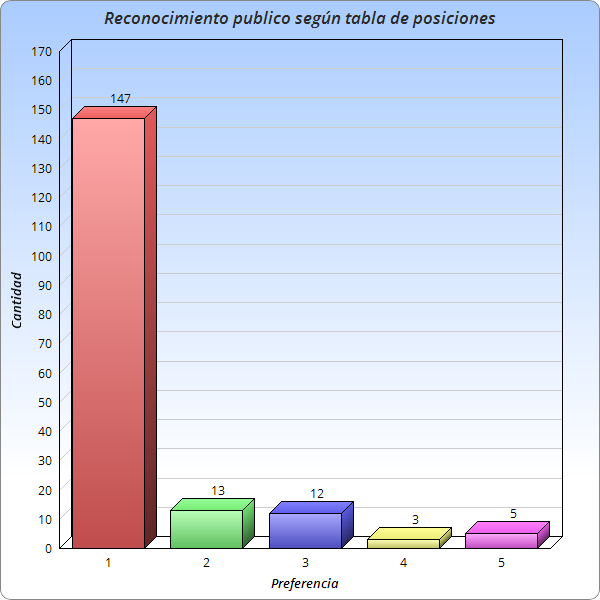
\includegraphics[width=0.6\textwidth]{images/Graficos/graf_5_8.png}
  \caption[Gráfico pregunta 7, cantidad de preferencias a beneficio de reconocimiento
publico según tabla de posiciones.]{Respuesta a pregunta 7, cantidad de preferencias a beneficio de reconocimiento
publico según tabla de posiciones.}
  \label{fig:chart5.8}
  %\url{http://www.chartgo.com/get.do?id=69b1dc7d4e}
\end{figure}

\begin{figure}[!htb]
  \centering
  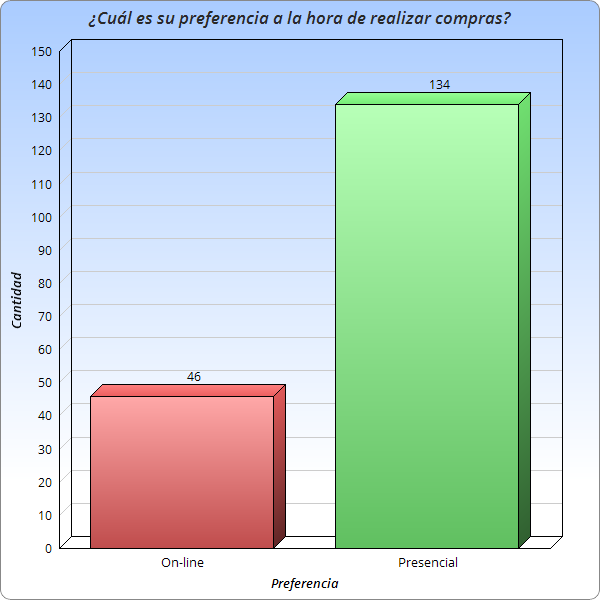
\includegraphics[width=0.6\textwidth]{images/Graficos/graf_5_9.png}
  \caption[Gráfico pregunta 8, preferencia al momento de comprar.]{Respuesta a pregunta 8, preferencia al momento de comprar.}
  \label{fig:chart5.9}
  %\url{http://www.chartgo.com/get.do?id=69b1dc7d4e}
\end{figure}

\begin{figure}[!htb]
  \centering
  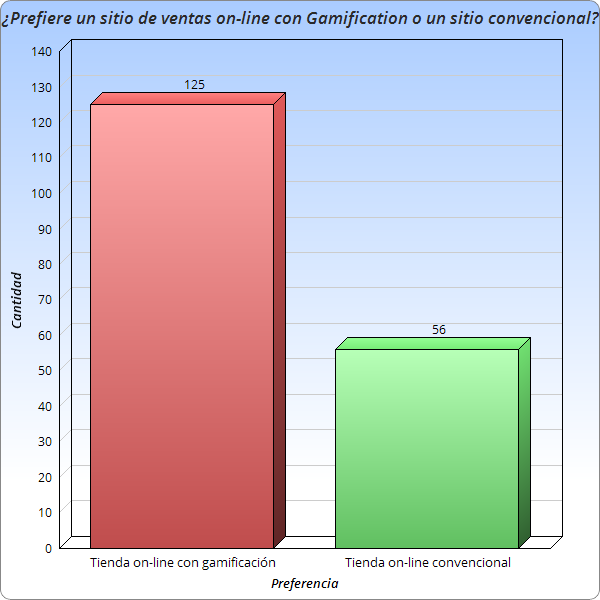
\includegraphics[width=0.6\textwidth]{images/Graficos/graf_5_10.png}
  \caption[Gráfico pregunta 9, preferencia al momento de comprar de forma \emph{on-line}.]{Respuesta a pregunta 9, preferencia al momento de comprar de forma \emph{on-line}.}
  \label{fig:chart5.10}
  %\url{http://www.chartgo.com/get.do?id=69b1dc7d4e}
\end{figure}

\begin{figure}[!htb]
  \centering
  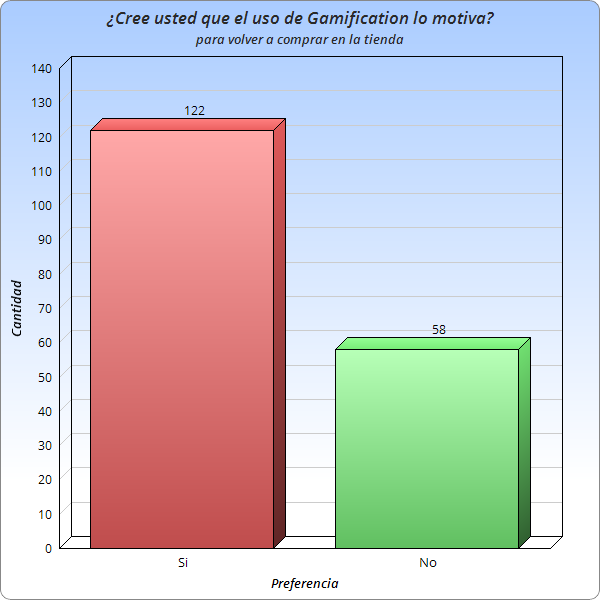
\includegraphics[width=0.6\textwidth]{images/Graficos/graf_5_11.png}
  \caption[Gráfico pregunta 10, motivación para volver a comprar en una misma tienda.]{Respuesta a pregunta 10, motivación para volver a comprar en una misma tienda.}
  \label{fig:chart5.11}
  %\url{http://www.chartgo.com/get.do?id=69b1dc7d4e}
\end{figure}

\begin{figure}[!htb]
  \centering
  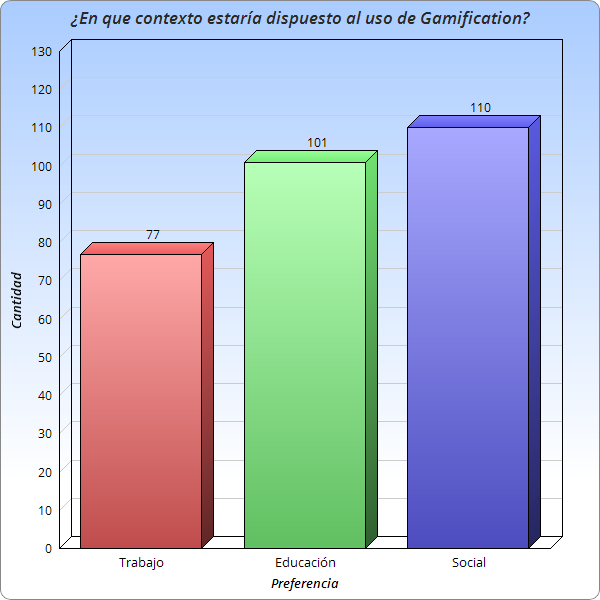
\includegraphics[width=0.6\textwidth]{images/Graficos/graf_5_12.png}
  \caption[Gráfico pregunta 11, contextos a los cuales se le podría implementar {\gam}.]{Respuesta a pregunta 11, contextos a los cuales se le podría implementar {\gam}.}
  \label{fig:chart5.12}
  %\url{http://www.chartgo.com/get.do?id=69b1dc7d4e}
\end{figure}


